% vim: tw=78 encoding=utf8 ts=2 sw=2 expandtab softtabstop=2
\documentclass[11pt,twocolumn,a4paper,english]{article}

% Evaluation of software clustering algorithms is typically done by comparing the clustering results to an authoritative decomposition prepared manually by a system expert. (Shtern, Tzerpos - On the Comparability of Software Clustering Algorithms)

% textmate: cmd+shift+; > change language to english > cmd+option+; (twice)

\usepackage[utf8]{inputenc}
\usepackage{babel}
\usepackage{url}
\usepackage{graphicx}
\usepackage{amsmath}
\usepackage{amssymb}
\usepackage{framed}
\usepackage{anysize}
\marginsize{1.7cm}{1.7cm}{1.7cm}{1.7cm}

\newcommand{\TODO}{\textbf{TODO:} }

\title{
Synthetic Benchmarks for Architecture Recovery Algorithms}
\author{Rodrigo Souza \\ rodrigorgs@gmail.com 
\and Dalton Guerrero \\ dalton@dsc.ufcg.edu.br
\and Jorge Figueiredo \\ abrantes@dsc.ufcg.edu.br
\and Christina Chavez \\ flach@ufba.br
}

\begin{document}

\sloppy
\maketitle

\tableofcontents
% \line(1,0){8.2 cm}
\vspace{1 em}

\TODO Add configurations for $G$ in the experiment

\TODO Maybe add borders to (at least some) figures.

\TODO Redo some figures to fit better in a two column paper.

\TODO Display authors in a 2x2 matrix.

\TODO \textbf{Static} dependency graphs

% \TODO Maybe put section ``The BCR+ Model'' after ``Software-Realism'' and before ``BCR+ Evaluation'', then move ``Triad Concentration Profiles'' to ``Background''. Maybe ``Related Work'' after ``Background''. The outline would become the following: Introduction, Background, (Related Work)?, Software-Realism, The BCR+ Model (includes description and evaluation), Evaluation of Architecture Recovery Algorithms.

% TODO entrada do BCR+ é uma arquitetura de referência.

\begin{abstract}
	As a software system evolves, its actual architecture may deviate from its original reference architecture. A better understanding of the actual architecture can be gained by applying architecture recovery algorithms to the source code of the system. Unfortunately, there is little knowledge regarding the quality of such algorithms, mostly because, in order to assess their accuracy, one needs updated, detailed architectures for a variety of software systems.
	To overcome such problem, we propose a simulation model that synthesizes implementation-level dependency graphs that conform to the module view of any given reference architecture. We show, using observations from network theory, that these graphs are very similar to dependency graphs extracted from the source code of real software systems. 
	Then, we synthesize thousands of graphs, in a controlled way, and use them as benchmarks for six well-known architecture recovery algorithms: ACDC, Bunch, SL75, SL90, CL75, and CL90. By comparing the given reference architectures with those recovered by the algorithms, we conclude that ACDC and Bunch outperform the alternatives, specially if the architecture contains more than a couple of modules. REVER EXPRESSAO.\end{abstract}

%%%%%%%%%%%%%%%%%%%%%%%%%%%%%%%%%%%%%%%%%%%%%%%%%%%%%%%%%%%%%%%%%%%%%%%%%%%%%
%%%%%%%%%%%%%%%%%%%%%%%%%%%%%%%%%%%%%%%%%%%%%%%%%%%%%%%%%%%%%%%%%%%%%%%%%%%%%

% I use begin/end instead of just \section so I can fold sections in my text editor
\begin{section}{Introduction}
% This section should be succinct, with no subheadings

	\begin{itemize}
		\item Recovery of reference architectures with the help of architecture recovery algorithms. 
		\item One kind of architecture recovery algorithms are software clustering algorithms (graph-based),  used to
recover module views.
		\item Not enough knowledge about performance of such algorithms.
		\item One reason: difficult to find documented architectures for a variety of different systems. Lack of benchmarks to test such algorithms.
		\item We propose (and evaluate) a model that synthesize graphs resembling software dependency graphs in a systematic way.
		\item Advantages: low cost (huge data sets), control over synthesis parameters.
		\item Results: we found such a model, evaluated it positively, and used it to do some analysis on architecture recovery algorithms.
		\item Structure of this paper. (First we devise a classifier do determine whether a graph is software-realistic)
	\end{itemize}
		
Architecture recovery algorithms have been used as a starting point to recover the reference architecture of a system family (Recovery of a Reference Architecture: A case study, by Eixelsberger / Architecture Recovery for Product Families, by Pinzger et al / Enhancing Domain-Specific Software Architecture Recovery, by Ivkovic and Godfrey) 
	([LIMBO] Improving the build architecture of legacy C/C++ software systems, by Dayani-Fard et al / [Bunch] ).
	
	One such kind of algorithms are the software clustering algorithms. They have been used mostly to recover module views of an architecture, that is, architectural documentation that comprises modules and their relationships [CITE]. These algorithms tend to find high cohesive clusters with low coupling between clusters. However, little is known about the performance of such algorithms on software. 
	
\end{section}

%%%%%%%%%%%%%%%%%%%%%%%%%%%%%%%%%%%%%%%%%%%%%%%%%%%%%%%%%%%%%%%%%%%%%%%%%%%%%

\begin{section}{Background and Related Work} \label{sec:back}
	\TODO Introductory paragraph. Why architecture recovery is important to our work. Why network theory is important.
	
	% \begin{itemize}
	% 	\item Architecture recovery (or discovery, or reconstruction). 
	% 	\begin{itemize}
	% 		\item Fully automated software clustering algorithms. ACDC, Bunch, Hierarchical.
	% 		\item Software dependency graphs.
	% 		\item Evaluation of software clustering algorithms (authoritativeness criterion).
	% 		\item Comparison between architectures (MoJoSim metric).
	% 		\item Related work: package dependencies, random graphs, evaluating clustering algorithms with the LFR model.
	% 	\end{itemize}
	% 	
	% 	\item Network theory
	% 	\begin{itemize}
	% 		\item (For practical purposes, network means graph)
	% 		\item Definitions: vertex, edge, degree (in- and out-), degree distribution
	% 		\item Scale-free networks (power law degree distributions)
	% 		\item Scale-free networks in software systems
	% 		\item Triad concentration profiles. TCPs as signature for a domain. TCPs in software. 
	% 	\end{itemize}
	% \end{itemize}

\begin{subsection}{Architecture Recovery}
	
	Software architecture recovery---also known as software architecture discovery/reconstruction---is a branch of reverse engineering that seeks tools, methods, and techniques to infer the architecture (or parts of it) for a software system by analyzing artifacts such as source code or execution traces.
%
%When designing the architecture of a software system, the module viewpoint plays a major role, by specifying the modules of the system and their inter-relationships. Constraining such dependencies benefits the maintainability, portability, and reusability of the software system.	
	
	There are many kinds of architecture recovery tools and techniques. For an overview, we refer the reader to a taxonomy by Pollet and colleagues \cite{Pollet2007}.
In this paper, we are interested in software clustering algorithms that work on design extracted from source code through static analysis
to recover module views. 
Automated tools take as input a graph representing dependencies between source code entities (e.g., classes in a object-oriented software), and outputs a clustering of the entities (i.e., a set of clusters, so that each entity belongs in exactly one cluster). Each cluster can be interpreted as a module in the recovered architecture and the set of clusters can be regarded as a recovered module view of the implementation [CITE]. REVISAR.

	The recovered architecture seldom matches exactly the actual architecture. Nevertheless, it can be used a starting point to identify the actual modules and the entities that belong in each module. 
%
	An important criterion, therefore, to evaluate a software clustering algorithm is to what extent it produces clusterings that resemble the actual architectures of the systems being analyzed. Some authors call this criterion \textit{authoritativeness} [CITE].
	
	There are two issues that should be handled when performing authoritativeness evaluations:
the quantitative comparison of the recovered architecture with the reference architecture, and 
the identification of systems with updated and high-quality architecture information to be used as authoritative clustering.
	
	In this research, to tacle the first issue, that is, to quantitatively compare the recovered architecture with the reference architecture, we use MoJo [Tzerpos AND Holt]. To measure the similarity between clusterings, we use MoJoSim \cite{Bittencourt2009}.
%, a metric that has been used in software clustering studies. 
MoJoSim measures, in a scale from 0.0 to 1.0, the effort needed to transform the recovered clustering into the reference clustering, where 1.0 means no effort (that is, the clusterings are identical).
	
	The idea behind MoJoSim is that any clustering can be transformed into another by means of two operations: move and join. The move operation implies that one object is moved from its cluster to another cluster (existing or new). The join operation means that two clusters are joined together, giving rise to a new cluster that contains objects from both clusters. Note that there is no split operation: if a cluster is to be divided in two parts, this can be accomplished only by performing several moves.
	
	The count of moves and joins needed to transform the recovered clustering, $X$, to the reference clustering, $Y$ is called the MoJo between the clusterings. MoJoSim is computed by normalizing MoJo to a 0.0---1.0 range:
	
	$$
	\mathrm{MoJoSim}(X, Y) ~=~ 1 - \frac{\mathrm{MoJo}(X, Y)}{n}\mathrm{,}
	$$
where $n$ is the number of objects (vertices) in the clustering.
	
	There are different approaches that address the second issue, that is, the identification of systems with updated and high-quality architecture information, ready to be used as authoritative clustering.
	
	The authoritative decomposition can be produced by a human architect, expert in the target system(s). High cost.
	
	Some studies use the structure of the source code folder as the authoritative architecture \cite{Bittencourt2009,Wu2005}.
	
	Other studies produce random graphs \cite{Mitchell2007}.  As the network science shows, random graphs are not realistic representations of software systems (see next section).
	
\end{subsection}

\begin{subsection}{Network Theory}
	
	Network theory (or network science) is an interdisciplinary field concerned with the study of networks (i.e., sets of interconnected objects). It does so by combining knowledge from statistics, physics, computer science, social network analysis and many other disciplines.

	Some authors distinguish between networks and graphs, by using the term graph to mean an abstract, formal representation of a network. However, this distinction is not universally accepted, so, for our purposes, graph and network can be used interchangeably.

	\TODO Instead of one paragraph explaining all concepts, may define as they are used.
	Some concepts from graph theory should be familiar to most readers with computer science background. A graph is a set of vertices and edges, where each vertex represents a relationship between two vertices. An edge can be either directed---meaning that there is an origin and a destination vertices---or undirected---meaning that the relationship between vertices is symmetrical. The degree of a vertex is the number of edges connected to it. The in-degree of a vertex is the number of edges that have the vertex as the destination (ingoing edges) and, similarly, the out-degree of a vertex is the number of edges that have the vertex as the origin (outgoing edges).

\begin{subsubsection}{Degree Distribution}
	One of the main results in network theory refers to the distribution of vertex degrees in commonly studied domains. Previously, it was believed that, in most domains, %the interconnection of objects was normally distributed (or formally, that 
the distribution of vertex degree followed a normal distribution.%). 
According to this mindset, every person had approximately the same amount of friends---some more, some less, but the exact value oscillated around a mean value---, every webpage had approximately the same amount of links, and so on. 
%	
	This pattern can be approximated by the random graph model \cite{Erdos1959}. \TODO describe
	
	However, % it was discovered that 
	many graphs that emerge from the interaction between real-world objects---including friendship graphs, web graphs, protein interaction graphs, and many others---do not present normally distributed degrees [CITE]. In the so-called scale-free graphs, the number of vertices connected to exactly $k$ other vertices---represented as $\mathrm{N}(k)$---is given by a power law, that is, $\mathrm{N}(k)$ is proportional to $k^{-\alpha}$, where $\alpha$ is a constant typically between 2 and 3.
	
	Scale-free graphs have been found thoroughly in software artifacts. They have been found in UML diagrams \cite{Valverde2003}, function calls, aggregation and inheritance relationships in C and C++ programs \cite{Myers2003}, in implementation-level dependencies for programs written in Smalltalk and Java \cite{Marchesi2004,Concas2007,Hyland-Wood2006,Baxter2006,Ichii2008}, in dependencies between software packages \cite{Labelle2004} and between dynamic libraries \cite{Louridas2008} and in runtime references between objects \cite{Potanin2005}.	
\end{subsubsection}

	\begin{figure*}[tbp]
		\centering
			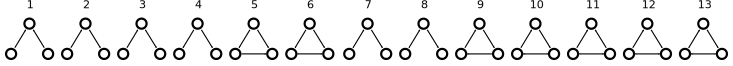
\includegraphics[scale=1]{figures/triads}
		\caption{All triads---connected directed graphs with three vertices---, numbered from 1 to 13.}
		\label{fig:triads}
	\end{figure*}
	
\begin{subsubsection}{Triad Concentration Profiles}
	In addition to degree distribution, graphs can be characterized by triad concentration profiles. Given three vertices, one can conceive 13 distinct connected directed graphs---the so-called triads---, as shown in Figure \ref{fig:triads}. By counting how often each triad appears in a graph, one can build a 13-dimension vector that is called the triad concentration profile for that particular graph. % it's like the signature for a graph.

	\begin{figure*}[htbp]
		\centering
			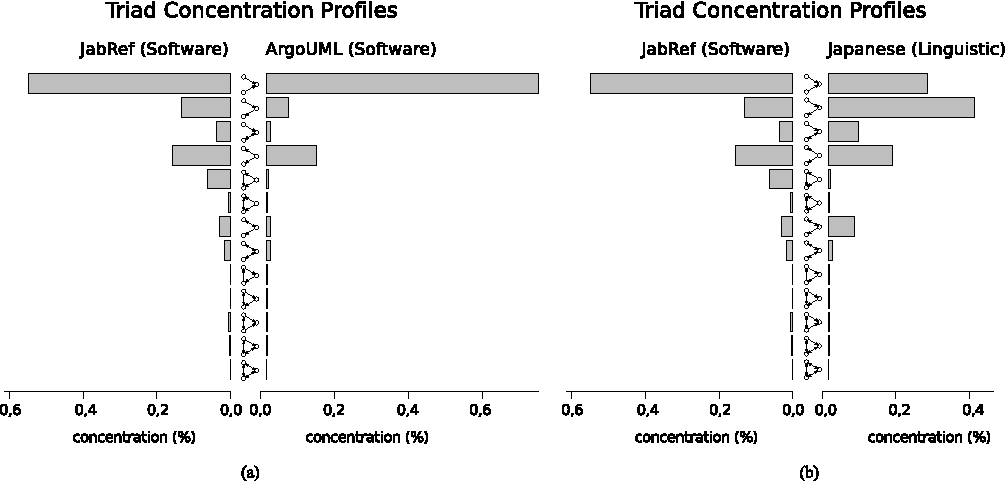
\includegraphics[scale=1]{figures/tcp}
		\caption{Comparison between triad concentration profiles for three distinct graphs (computed with the igraph tool \cite{igraph}). (a) Class dependency graphs for two softwares: JabRef, version 2.5b2 (left) and ArgoUML version 0.28 (right). (b) Graph for JabRef, version 2.5b2 (left), and graph of word succession in a sample of Japanese texts (right) \cite{Milo2004}.}
		\label{fig:tcp}
	\end{figure*}
	
	Previous work has shown that graphs from the same domain tend to be characterized by similar triad concentration profiles \cite{Milo2002}. For example, Figure \ref{fig:tcp}(a) presents triad concentration profiles for two software dependency graphs, whereas Figure \ref{fig:tcp}(b) presents triad concentration profiles for graphs in distinct domains: a software dependency graph and a linguistic graph. An informal analysis reveals that the similarity between the profiles is greater in the first case. It should suffice to notice that, in the second case, the concentration of the first two triads is somewhat reversed (in the linguistic graph, the second triad is the most frequent). EXPLICAR MELHOR.



	Many authors \cite{Milo2004,Ma2007,Lin2008} have explored triad concentration profiles as a means to find clusters of structurally similar graphs. The results suggest that such profiles can be effectively used to identify groups of graphs from the same domain (e.g., social, linguistic, biologic etc.).
\end{subsubsection}
	
	% \begin{itemize}
	% 	\item (For practical purposes, network means graph)
	% 	\item Definitions: vertex, edge, degree (in- and out-), degree distribution
	% 	\item Scale-free networks (power law degree distributions)
	% 	\item Scale-free networks in software systems
	% 	\item Triad concentration profiles. TCPs as signature for a domain. TCPs in software. 
	% \end{itemize}
	
\end{subsection}


\end{section}

%%%%%%%%%%%%%%%%%%%%%%%%%%%%%%%%%%%%%%%%%%%%%%%%%%%%%%%%%%%%%%%%%%%%%%%%%%%%%

% \begin{section}{Proposed solution}
% 	\TODO move to introduction
% 	Goal: analyze or compare architecture recovery algorithms in different contexts.
% 	
% 	Research approach:
% 	
% 	\begin{itemize}
% 		\item Create a model that synthesizes graphs that are similar to software dependency graphs, given a reference architecture
% 		
% 		\begin{itemize}
% 			\item Create a graph classifier, that determines if a graph is likely to be a software dependency graph (i.e., if it is software-realistic)
% 			\item Evaluate the classifier, in terms of precision and recall
% 			\item Using the classifier, determine if the model synthesizes software-realistic graphs 
% 		\end{itemize}		
% 	\end{itemize}
% 	
% 	Usage (exemplified in our proof of concept):
% 	
% 	\begin{itemize}
% 		\item Use the model to synthesize a variety of graphs. 
% 	
% 		\item Apply architecture recovery algorithms to the graphs.
% 	
% 		\item Compare recovered with reference architectures.
% 	
% 		\item Analyze.
% 	\end{itemize}
% 	
% 	
% \end{section}

%%%%%%%%%%%%%%%%%%%%%%%%%%%%%%%%%%%%%%%%%%%%%%%%%%%%%%%%%%%%%%%%%%%%%%%%%%%%%

\begin{section}{Software-Realism Classifier} \label{sec:sr}
	% Motifs / Triads. Triad concentration profiles.
	% Software-realism metric.
	% Software-realism classifier. Training and testing the classifier.
	% Software-realism for the BCR+ model. (Cite previous paper, where we also evaluate software-realism for three other models)

	If synthetic graphs are to be used as surrogates to dependency graphs extracted from the source code of software systems, it is expected that they resemble such graphs. The property of a graph to resemble software dependency graphs is what we call software-realism. Hence, we seek a method to determine whether any given graph is software-realistic. %Hence, we seek to prove that BCR+ produces software-realistic graphs.
	
	To this end, we propose a software-realism classifier that, given a graph, outputs whether it is software-realistic or not (i.e., whether it is likely that the graph represents dependencies in a software system). Then, we show that this classifier presents high precision and high recall, and thus is able to discriminate between both classes of graphs. %Finally, we conclude that BCR+ is able to synthesize software-realistic graphs, indistinguishable from software dependency graphs.
		
\begin{subsection}{Method}

In order to build a classifier to discriminate between software-realistic and non software-realistic graphs, we have to chose properties from graphs that can help in such distinction. We have chosen triad concentration profiles, because previous literature suggests that specific patterns in such profiles correspond to well-defined problem domains \cite{Milo2004}.

Therefore, our classifier should take as input the triad concentration profile of a graph and output its more probable class (software-realistic or non software-realistic). We can formalize the classifier as a function with one binary output:

$$
  \mathrm{S}(t_1, \ldots, t_{13}) = \left\{ \begin{array}{rl}
	 1 &\mbox{ if software-realistic} \\
	 0 &\mbox{ otherwise,}
	       \end{array} \right.
$$
where $t_1, \ldots, t_{13}$ are the relative frequencies of the 13 triads in the input graph, i.e., the triad concentration profile for the graph.

To build the classifier, a  supervised learning method is used; the classifier is trained by being supplied with instances of graphs from both software-realistic and non software-realistic classes. Because the software-realism is not an objective property of a graph, in our work we decided to treat any software dependency graph as software-realistic, and any graph from other domains as non software-realistic.

The supervised learning method used was the logistic regression classifier, due to its simplicity. The model for a logistic regression classifier is based on the sigmoid function:

$$
	\mathrm{f}(t_1, \ldots, t_{13}) = \frac{1}{1 + e^{-z}}\mathrm{,}
$$
where $z$ is given by

$$
  z = \alpha_0 + \alpha_1t_1 + \cdots + \alpha_{13}t_{13}
$$

The function $\mathrm{f}$ yields the probability that the provided graph belongs to class 1 (software-realistic). A simple rounding is then used to transform this output in one of the classes ($\{0, 1\}$):

$$
\mathrm{S}(t_1, \ldots, t_{13}) = \left\{ \begin{array}{rl}
 1 &\mbox{ if } \mathrm{f}(t_1, \ldots, t_{13}) \ge 0.5 \\
 0 &\mbox{ otherwise}
       \end{array} \right.
$$
% 
% We propose a classifier, based on triad concentration profiles, that, given a graph, determine if it is software-realistic (i.e., if it is likely to be a software dependency graph). In other words, we consider two classes of graphs---software-realistic and non software-realistic---, and build a model that determines the class of any given graph. 
% 
% The classifier is developed by training a logistic regression model on a data set containing both software and non-software graphs. We show that it is capable of correctly classifying most graphs.

\begin{subsubsection}{Data Set} \label{sec:data-set}
	
	In order to train our classifier, we have collected 131 graphs, including 65 software dependency graphs (software-realistic) and 66  directed graphs from other domains (non software-realistic).
	
	The collected 66 non software-realistic graphs were made available by researchers working on domains such as biology, sociology, technology, and linguistics. The size of these graphs range from 32 to 18,163 vertices. The complete list of graphs can be found in Appendix A. \TODO Create Appendix
	
	Also, we have collected 65 open source software systems written in Java and listed at SourceForge.net\footnote{\url{http://sourceforge.net/about}} among the most popular as of 2008. From each software system one dependency graph was extracted, as follows.
	
	The archive for each software system contained one or more JAR files (Java Archive), with object code for each class or interface. Some JAR files were generic libraries used by the systems; these files were removed from the extraction, as they are not really part of the software.
To extract dependencies between classes (or interfaces) from the remaining JAR files, we used Dependency Finder\footnote{\url{http://depfind.sf.net/}}, a tool with command-line interface that enables its integration in scripting environments. %We believe that any other tool with the same purpose would produce similar outputs.
	
	The graphs that were extracted contain vertices representing Java classes and interfaces. The edges represent any reference from one class/interface to another in the object code, including inheritance, aggregation, method call, object instantiation and attribute read/write.
	
	After the extraction process, we ended up with 65 software dependency graphs, with sizes ranging from 63 to 6,433 vertices. More information about these graphs can be found in Appendix A. % TODO
	
	For each of the 131 graphs, we extracted its triad concentration profile using the tool igraph \cite{igraph}. No other information about the network (such as number of vertices or number of edges) was used to build the classifier.

\end{subsubsection}

\begin{subsubsection}{Training and Testing}
	
	The data set with 131 graphs (65 software dependency graphs, 66 graphs from other domains) was used to train a logistic regression classifier using the data mining tool Weka \cite{weka}. To this end, we considered that software dependency graphs are software-realistic, and the other graphs are not. 
		
	First, we trained the logistic regression model on the full data set with 131 graphs. After the training, the logistic regression classifier was tested on the same 131 graphs, being able to correctly classify 129 of them. Of course, this result is not an accurate estimation of the performance of the classifier, since the same data set was used for training and for testing.
	
	In order to assess how well the graph classification could perform on an independent data set, we used the method of 10-fold stratified cross-validation. In this method, the data set is first split randomly in 10 folds (or partitions). The folds are stratified, that is, in each fold, the distribution of classes should match approximately that of the full data set. In our data set, it means that each fold should contain approximately $\frac{65}{131} = 49.6\%$ of software-realistic graphs. 
	
	The cross-validation is performed in 10 iterations. In each iteration, one fold is chosen as the test set, and the remaining ones, combined, form the training set. This way, in each iteration, a classifier is trained on 90\% of the data set and tested on the other 10\%. It should be noted that each data set instance is used exactly once for testing. Because of this, we can compare the real and the predicted class for each instance, and then compute standard performance metrics such as precision and recall. 
	
	Let $S$ be the set of all software-realistic graphs from our data set (that is, all graphs that were extracted from software systems), and let $L$ bet the set of networks predicted by the classifier to be software-realistic. The precision is, then, given by
	
	$$
	\mathrm{precision}: ~\frac{|S \cap L|}{|L|},
	$$
and the recall is given by
	
	$$
	\mathrm{recall}: ~\frac{|S \cap L|}{|S|}.
	$$
	
	Intuitively, the precision is the proportion of graphs predicted as software-realistic that are indeed software-realistic. Recall is the proportion of software-realistic graphs that are correctly predicted by the classifier. A good classifier should have high precision and high recall.
	
\end{subsubsection}

\begin{subsubsection}{Results}
	
	We evaluated the precision and recall of the graph classifier using the previously explained 10-fold cross-validation method, obtaining 92.6\% precision and 96.9\% recall. The high values suggest that the classifier is able to identify most software dependency graphs and also that it misclassifies only few graphs.

\begin{framed}
The software-realism classifier is very accurate, with 92.6\% precision and 96.9\% recall.	
\end{framed}
	
% \fbox{
% \parbox{0.85\linewidth}{
% }
% }
	
	The model is the following:
% 
% \begin{framed}
% 	\begin{array}{rl}
% 	 z = & 0.09 \\
% 	     & + 6.67t_1 \\
% 	     & - 10t_2 \\
% 	     & - 9.46t_3 \\
% 	     & + 5.73t_5 \\
% 	     & + 40.3t_6 \\
% 	     & + 23.45t_7 \\
% 	     & - 157.7t_{10} \\ 
% 	     & - 138.36t_{12} \\
% 	     & - 843.11t_{13}\mathrm{,}
% 	\end{array}
% 	
% \end{framed}


\begin{framed}
$z = 0.09 + 6.67t_1 - 10t_2 - 9.46t_3 + 5.73t_5 + 40.3t_6 + 23.45t_7 -157.7t_{10} -138.36t_{12} - 843.11t_{13}$
\end{framed}
% where $t_i$ is the relative frequency of the $i$-th triad. 
	
	The results show that we can determine with high confidence whether a graph is software-realistic by looking at its triad concentration profile (to be precise, by looking at the concentration of 9 out of the 13 triads). The implications are that synthetic graphs can be used in studies that rely on software dependency graphs, as long as the synthetic graphs are classified as software-realistic.


\end{subsubsection}

\end{subsection}
	
\end{section}

%%%%%%%%%%%%%%%%%%%%%%%%%%%%%%%%%%%%%%%%%%%%%%%%%%%%%%%%%%%%%%%%%%%%%%%%%%%%%

\begin{section}{The BCR+ Model}	\label{sec:bcr}
	\newcommand{\din}[0]{\ensuremath{\delta_{in}}}
	\newcommand{\dout}[0]{\ensuremath{\delta_{out}}}
	\newcommand{\gin}[0]{\ensuremath{\mathrm{d}_{in}}}
	\newcommand{\gout}[0]{\ensuremath{\mathrm{d}_{out}}}
	
	In this section, we describe the BCR+ model for synthesizing graphs from a description of the module viewpoint of an arbitrary architecture --- that is, the modules and dependencies between modules. The BCR+ model produces---by means of the mechanisms of growth and preferential attachment---directed graphs that are both scale-free and segmented in modules.
	
	\TODO as far as we know it is the only graph model that takes module dependencies as input.
	
	Then, we evaluate graphs synthesized by BCR+ using the previously described software-realism classifier. We conclude that BCR+ is able to synthesize software-realistic graphs, indistinguishable from software dependency graphs. \TODO we should also argue in favor of its software-realism by saying that it produces scale-free graphs.
	
	\TODO there are other models, but they don't take architecture as input	
	
\begin{subsection}{Overview}
	The BCR+ model is a generalization of a graph model proposed by Bollobás et al \cite{Bollobas2003}. The original model generates directed graphs that are scale-free. Our model extends the original by generating graphs in which the nodes are organized in modules, according to an modular architecture given as input.
	
	\TODO BCR+ is a growth model, can simulate the evolution of a software system subject to constraints in module interaction. See CSMR paper (extended version), pg 2, col 2, just before section B. 
	
	The BCR+ model takes the following parameters as input:
	
	\begin{itemize}
  \item number of vertices, $n$;
  \item three probability values, $p_1$, $p_2$ e $p_3$, com $p_1 + p_2 + p_3 = 1$;
  \item base in-degree, $\din$;
  \item base out-degree, $\dout$.
  \item an directed graph representing dependencies between modules, $G$;
  \item a constant, $\mu$, with $0.0 \le \mu \le 1.0$;
  \end{itemize}
  
	The last two parameters are new in BCR+. The other ones are from the original model by Bollobás et al \cite{Bollobas2003}.
	
	In the graph $G$, each vertex represents one module of the architecture. Each edge defines a relationship of dependency between modules. We say that a module $M_1$ depends on another module, $M_2$, if $G$ contains an edge from the vertex that represents $M_1$ to the vertex that represents $M_2$. In the graph that is created, an edge from a vertex $v_1 \in M_1$ to another vertex, $v_2 \in M_2$, can be created only if $M_1$ depends on $M_2$ in the graph $G$ or if $M_1$ and $M_2$ are the same module.
	
		\TODO Say that these graphs contain both internal and external edges. Define internal/external.
		
	The parameter $\mu$ controls the proportion of external edges in the graph---that is, edges connecting vertices in distinct modules. Lower values lead to graphs with fewer external edges.
	
	The original model by Bollobás et al \cite{Bollobas2003} is a particular case of BCR+ when $\mu = 0$ and $G$ contains one single vertex, representing one single module.
	

\begin{figure*}[htbp]
	\centering
		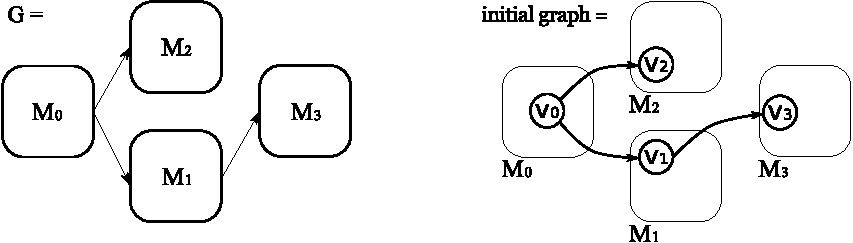
\includegraphics[scale=1]{figures/bcr-initial-graph}
	\caption{Initial graph synthesized by BCR+, given an input graph parameter $G$.}
	\label{fig:bcr-initial-graph}
\end{figure*}
	
	As a computer model, BCR+ takes the parameters as inputs and, by running an algorithm, outputs a graph. The algorithm builds the output graph incrementally. It starts by creating a module for each vertex in the input graph $G$, and then adding one vertex to each module. After that, it creates all external edges that are allowed by $G$ (see Figure \ref{fig:bcr-initial-graph}). Then, the graph is modified according to three formation rules that are applied successively, in random order, until the graph grows to $n$ vertices. At each algorithm step, the probability of the $i$-th being applied is given by the parameter $p_i$.

\end{subsection}	

\begin{subsection}{Formation Rules}
	
	There are three formation rules in BCR+. Each one modifies the output graph by adding or removing vertices or edges in the graph. Also, each formation rule has a probability of being applied, given by the parameters $p_1$, $p_2$ and $p_3$.

\begin{figure}[htbp]
	\centering
		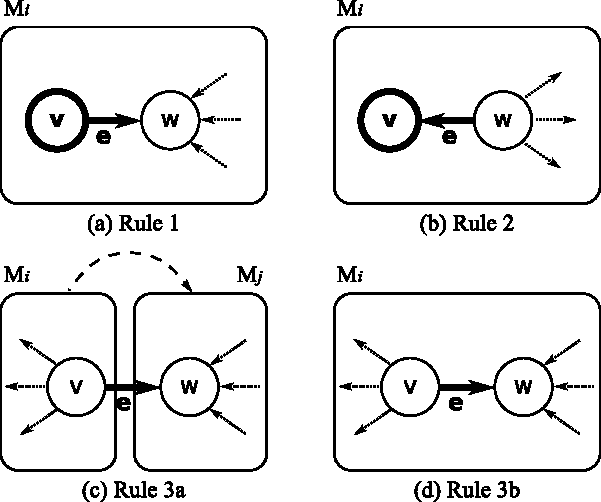
\includegraphics[width=0.45\textwidth]{figures/bcr-rules}
	\caption{Formation rules for BCR+. $M_i$ and $M_j$ are distinct modules, such as $M_i$ depends on $M_j$. In the diagram for each rule, thicker lines represent vertices and edges created when the rule is applied.}
	\label{fig:bcr-rules}
\end{figure}

	The rules are illustrated in Figure \ref{fig:bcr-rules}. Simplified rules:
	
	\begin{itemize}
		\item Rule 1: one vertex is added to some module, together with an outgoing edge to another vertex in the same module.
		\item Rule 2: one vertex is added to some module, together with an ingoing edge coming from another vertex in the same module.
		\item Rule 3: one edge is added between two pre-existing vertices. There are two variations of this rule:
		\begin{itemize}
			\item Rule 3a: choose vertices from distinct modules.
			\item Rule 3b: choose vertices that are in the same module.
		\end{itemize}
	\end{itemize}
	
	% The rules 1, 2, and 3b come directly from the original model by Bollobás et al \cite{Bollobas2003}. The rule 3a was created in BCR+ to account for inter-module dependencies.
	
	The choice of vertices to which add edges to is done according to preferential attachment. When we say that a vertex ``chosen according to $\mathrm{f}(x)$'', we mean that the probability of choosing the vertex $x$ is proportional to $\mathrm{f}(x)$:
	
	$$
	  \mathrm{P}(x) ~=~ \frac{ \mathrm{f}(x) }
	  { \displaystyle\sum_{i} \mathrm{f}(i) }
	$$
	
	The denominator is a normalization factor, such as the sum of probabilities $\mathrm{P}(x)$ is 1.
	
	With this definition in mind, the rules can be fully specified:
	
	\begin{itemize}
		\item Rule 1: \emph{Add a vertex with an outgoing edge}. An existing vertex, $w$, is chosen according to $\mathrm{f}(x) = \din + \gin(x)$ (that is, parameter $\din$ added to the vertex in-degree). A new vertex, $v$, is added to the module that contains $w$, together with an edge from $v$ to $w$.

		\item Rule 2: \emph{Add a vertex with an ingoing edge}. An existing vertex, $w$, is chosen according to $\mathrm{f}(x) = \dout + \gout(x)$. A new vertex, $v$, is added to the module that contains $w$, together with an edge from $w$ to $v$.

		\item Rule 3: \emph{Add an edge between pre-existing vertices}. A vertex, $v$, is chosen according to $\mathrm{f}(x) = \dout + \gout(x)$. Then, an edge is added from $v$ to another vertex, $w$, chosen according to $\mathrm{f}(x) = \din + \gin(x)$. The vertex $w$ is not chosen among the set of all vertices. In fact, there are two rules, and the choice of the rule to apply is probabilistic and depends on the parameter $\mu$:

		\begin{itemize}
		  \item Rule 3a: with proability $\mu$, $w$ is chosen among the vertices that are in modules on which the module of $v$ depends, according to the parameter $G$.
		  \item Rule 3b: with probability $1 - \mu$, $w$ is chosen among the vertices that are in the same module as $v$.
		\end{itemize}
	\end{itemize}
		
\end{subsection}

\begin{figure*}[htbp]
	\centering
		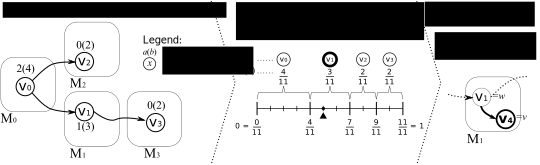
\includegraphics[width=\textwidth]{figures/bcr-example}
	\caption{One step of BCR+.}
	\label{fig:bcr-example}
\end{figure*}

\begin{subsection}{Example} \label{sec:example}
	
	To illustrate the behavior of BCR+, we show in Figure \ref{fig:bcr-example} one step of graph synthesis process. Suppose that we chose $G$ to be the four-module graph from Figure \ref{fig:bcr-initial-graph}, so the first step is to create one vertex for each module and then connect them according to the edges in $G$. 
	
	Now, suppose that $\dout = 2$ and that rule 2 was chosen. In this case, a vertex must be chosen, and this choice must consider, for each vertex, $x$, the value of $\mathrm{f}(x) = \dout + \gout(x)$. In the figure, the value of $\mathrm{f}(x)$ for each vertex is represented by a number inside parentheses near the vertex (the number before the parentheses is simply $\gout(x)$, the out-degree of vertex $x$).
	
	Each vertex, $x$, has a probability $\mathrm{P}(x)$ of being chosen, where $\mathrm{P}(x) = \frac{\mathrm{f}(x)}{\sum_i \mathrm{f}(i)}$. In this particular example, $\mathrm{P}(x) = \frac{\mathrm{f}(x)}{11}$, so that the sum of all probability values equals 1.0.
	
	The probability values associated with each vertex can be represented by the real line shown in the center of Figure \ref{fig:bcr-example}. Each vertex occupies a segment in the line that is proportional to the probability of it being chosen. The choice of the vertex is made by picking at random a real number between 0.0 and 1.0, marking it in the line and analyzing in which segment it falls. In the example, the value $\frac{5}{11}$ was chosen, which corresponds to a point of the segment of $v_1$ in the line. After the vertex $v_1$ was chosen, rule 2 determines that a new vertex (we can call it $v_4$) is added to $M_1$ (the module that contains $v_1$), together with an edge from the chosen vertex, $v_1$, to newly created vertex, $v_1$.
	
	It should be clear that vertices with high out-degree are more likely to receive new outgoing edges. The parameter $\dout$ can be thought as a base out-degree that is added to all vertices when the probabilities are computed, thus rendering the probability distribution more homogeneous. In the present example, if $\dout$ was zero, vertices $v_2$ and $v_3$ could not be chosen, because both have zero out-degree. Of course, the same reasoning applies to $\din$ and the in-degree.

\end{subsection}
	
\begin{subsection}{BCR+ Evaluation}
	In the previous subsection, we have proposed a graph classifier that determine, with high precision and recall, whether a graph is software-realistic. In this section, we evaluate whether the BCR+ graph model is able to synthesize software-realistic graphs. The evaluation process is divided in three steps:
	
	\begin{enumerate}
		\item \emph{parameter selection}: by varying the values of the parameters of the model, we come to thousands of possible parameter configurations, so to explore the variety of graphs that can be synthesized;
		
		\item \emph{graph synthesizing}: for each parameter configuration, we synthesize three graphs, in order to mitigate the effect of randomness in the synthesis process;
		
		\item \emph{graph classification}: each graph is classified (using the previously built graph classifier) as software-realistic or non software-realistic.
	\end{enumerate}
	
\begin{subsubsection}{Parameter Selection}
	To synthesize a large variety of graphs, we have varied the value of each parameter from BCR+ so as to cover a wide range of possible values. Each assignment of values to parameters is called a configuration. We have chosen configurations for each possible combination of the selected parameter values.
		
	To recap, BCR+ has seven parameters: the number of vertices, $n$; the reference architecture, $G$; three complementary probabilities, $p_1$, $p_2$, and $p_3$; the mixing probability, $\mu$; and nonnegative values $\din$ and $\dout$. The probabilities are bounded parameters, with values ranging from 0.0 to 1.0. The remaining parameters are more complex.
	
	Because most parameters take real values as input, it is not possible to cover all possible values, so they have been split in discrete intervals. Also, to avoid combinatorial explosion, we have limited the configuration space to at most six values per parameter.
	
	We have fixed the number of vertices, $n$, to 1,000, a value that has been used in related work \cite{Lancichinetti2009b}. To fix the number of vertices should not influence the results, since it affects only the size of the graph, not the pattern of connections between vertices.
	
	The parameter $G$ is the most complex, because it determines not only the number of modules, but also the interconnection between these modules. It should be noted that, with only three modules, there are 13 possible values for $G$ in which no module is isolated from the others.
	
	In order to avoid arbitrary graphs for $G$, we have instead used graphs that were extracted from software systems from the data set described in section \ref{sec:data-set}. For this task, we have extracted dependencies for all JAR files bundled with the system, including library files. Then, we have considered that each JAR is a module and that dependencies from entities in one JAR to entities in another JAR represent dependencies between modules. We believe that JAR files are good surrogates to modules, because distinct JAR files usually correspond to the work of distinct development teams.
	
	In the end, 5 graphs were chosen as $G$, with sizes from 2 to 32 modules. The graphs were extracted from the following software systems: GEF (2 modules), iBATIS (4 modules), MegaMek (8 modules), findbugs (16 modules), and zk (32 modules).
	
	For the parameters $p_1$, $p_2$, and $p_3$, we have chosen values in the set $\{0.0, 0.2, 0.4, 0.6, 0.8, 1.0\}$, such as $p_1 + p_2 + p_3 = 1.0$. Also, we determined that $p_1 + p_2 > 0$, because $p_1$ and $p_2$ correspond to rules that add vertices (otherwise, the graph would not grow in number of vertices).
	
	For the parameter $\mu$, we have selected values from the set $\{0.0, 0.2, 0.4, 0.6\}$. Because $\mu$ controls the proportion of external edges, that connect vertices from distinct modules, we avoided high values, that would lead to highly coupled graphs.
	
	For the parameters $\din$ and $\dout$, we have selected values from the set $\{0, 1, 2, 3, 4\}$. The values are somewhat arbitrary, but we avoided high values, because they would render graphs in which the distribution of edges per vertex is more homogeneous, unlike the distribution for software dependency graphs.
	
	For the selected parameter values, there are 9,500 configurations.
	%For unbounded parameters, we have chosen values based on the literature or grounded in the observation of software dependency graphs.

\end{subsubsection}

\begin{subsubsection}{Graph Synthesis and Evaluation} \label{sec:bcr-synthesis}
	
	For each parameter configuration, three graphs were synthesized, using distinct random seeds for each generation. Therefore, there were 28,500 synthetic graphs. Next, we classified each graph using the previously present graph classifier.

	% , to determine whether at least some of the graphs are software-realistic. We did not expect all graphs to be software-realistic. Because the synthesis process and the graph classification are both fast (less than 1 second on a 2.2 GHz processor, with no code optimizations), we can synthesize a lot of graphs and filter out the ones that are not software-realistic, as long as there are at least some software-realistic graphs.
	
	A total of 10,000 (35.1\%) graphs were classified as software-realistic. Although the majority of the graphs synthesized by BCR+ do not resemble software dependency graphs, the results show that BCR+ is feasible for practical use. For any analyses that require software-realistic graphs, we can synthesize a large amount of graphs and filter out the ones that are not software-realistic, because both the synthesis and the classification process are fast (less than 1 second for each graph on a 2.2 GHz processor, using non-optimized code).

	For comparison, we also synthesized 1620 random directed graphs using a naive algorithm that keeps adding edges for randomly selected pairs of vertices until it reaches the desired number of edges \cite{Erdos1959}. We synthesized graphs with 1,000 vertices and the number of edges was chosen in the set $\{2,000; 2,100; \ldots ; 10,000\}$. For each value for the number of edges, 20 graphs were created. No graph from this set was classified as software-realistic. 
	
	The conclusion is that BCR+, together with the graph classifier, can be effectively used to synthesize graphs that resemble software dependency graphs. Also, we showed that naive graph synthesis algorithms, previously used in architecture recovery studies \cite{Mitchell2007}, are very unlikely to synthesize software-realistic graphs, even when a variety of parameter configurations is used.
	
	% \TODO histogram showing how many configurations had 3 software-realistic graphs (100\%), how many had 2 (66\%), how many had 1 (33\%), how many had 0. -- just out of curiosity
	
	% Build a predictor of the software-realism based on BCR+ parameters? -- maybe not, we already argued that synthesis + classification is fast.
	
\end{subsubsection}

\end{subsection}	
\end{section}

%%%%%%%%%%%%%%%%%%%%%%%%%%%%%%%%%%%%%%%%%%%%%%%%%%%%%%%%%%%%%%%%%%%%%%%%%%%%%

\begin{section}{Evaluation of Architecture Recovery Algorithms}
	\TODO Recap Bunch, ACDC, SL75, SL90, CL75, CL90; MoJo metric; experimental setup for evaluation of architecture recovery algorithms: given a dependency graph and a reference architecture, run the algorithm on the graph and compare the recovered architecture with the reference architecture.

\begin{subsection}{Experimental Setup}
	With the objective of comparing architecture recovery algorithms and understand the factors that affect their performance (how well they recover the reference architecture), three experiments were performed:
	
	\begin{itemize}
		\item the first one was aimed at comparing the performance of architecture recovery algorithms using the criterion of authoritativeness (how close the recovered architecture is from the reference architecture);
		\item the second one was aimed at understanding how the performance of the algorithms is affected by graph characteristics;
		\item the third one was aimed at assessing whether the presence of bidirectional intermodule dependencies poses a challenge to architecture recovery algorithms.
	\end{itemize}
	 
	Because the methods and data used in the three experiments are similar, we describe them together. The experiments consist of the following steps:
	
	\begin{enumerate}
		\item use BCR+ to synthesize graphs using many different parameter configurations;
		\item apply architecture recovery algorithms to each synthetic graph;
		\item measure the performance of the each algorithm in each graph (using the authoritativeness criterion);
		\item analyze the results using statistics.
	\end{enumerate}
	
	For the first step, we have used the synthetic graphs described in Section \ref{sec:bcr-synthesis}. The data set contains 28,500 graphs synthesized from 9,500 parameter configurations.
	
	We have chosen architecture recovery algorithms based on graph clustering that have free and publicly available implementations and that were studied by more than one author in papers about architecture recovery. By this criterion, we have selected the algorithms ACDC \cite{Tzerpos2000}, Bunch \cite{Mancoridis1998}, and hierarchical agglomerative clustering algorithms \cite{Anquetil1999}. For Bunch and ACDC, we used the default configurations provided by the original implementations provided by their respective creators.
		
	In the case of hierarchical algorithms, we have experimented with two linkage criteria---single-linkage (SL) and complete-linkage (CL)--and two height cutoff values---75\% and 90\%. There are, thus, 4 configurations for the hierarchical agglomerative algorithm, that will be referred as SL75, SL90, CL75, and CL90. These are the configurations studied by Anquetil  \cite{Anquetil1999,Anquetil2003} and then reproduced by others (e.g., \cite{Wu2005}).
	
	To measure the similarity between clusterings, we have chosen the metric MoJoSim \cite{Bittencourt2009}, that has been used in software clustering studies. MoJoSim measures, in a scale from 0.0 to 1.0, the effort needed to transform the recovered clustering into the reference clustering, where 1.0 means no effort (that is, the clusterings are identical).
	
	The idea behind MoJoSim is that any clustering can be transformed into another by means of two operations: move and join. The move operation implies that one object is moved from its cluster to another cluster (existing or new). The join operation means that two clusters are joined together, giving rise to a new cluster that contains objects from both clusters. Note that there is no split operation: if a cluster is to be divided in two parts, this can be accomplished only by performing several moves.
	
	The count of moves and joins needed to transform the recovered clustering, $X$, to the reference clustering, $Y$ is called the MoJo between the clusterings. MoJoSim is computed by normalizing MoJo to a 0.0---1.0 range:
	
	$$
	\mathrm{MoJoSim}(X, Y) ~=~ 1 - \frac{\mathrm{MoJo}(X, Y)}{n}\mathrm{,}
	$$
	
	where $n$ is the number of objects (vertices) in the clustering.
	
	Finally, we performed graphical analyses and hypothesis tests on the results. We have used non-parametric tests, because a preliminary analysis showed that the data are not normally distributed. In all experiments, the dependent variable is the performance (measured by MoJoSim) of a particular algorithm on the synthetic graphs.
	
\end{subsection}

\begin{subsection}{Comparison of Architecture Recovery Algorithms}
	% Section 6.4 from dissertation
	
	The first experiment was aimed at comparing the performance of the algorithms when applied software-realistic graphs, measured by the similarity between the clusters found by the algorithms and the modules of the reference architecture.
	
	We have selected for this experiment only the graphs that were classified as software-realistic, totalizing 10,000 graphs. Then, each algorithm was applied to each one of the synthetic graphs, resulting in a set of clusters together with a mapping from the set of vertices to the set of clusters. The performance of the clusterings were measured with the metric MoJoSim.
	
	The Figure \ref{fig:exp-algorithms} shows a box plot of the MoJoSim values that were measured for each algorithm. The dashed lines indicate the maximum and minimum value from the data. Comparing the median performance of the algorithms, it is clear that ACDC presents the best performance, followed by Bunch, and then by the hierarchical algorithms. These differences were verified to be significative by applying a paired Wilcoxon test ($\alpha = 0.05$), with Bonferroni correction to account for multiple hypothesis testing. Among the hierarchical algorithms, there was no evidence that their performances differ.
	
	\begin{figure}[htbp]
		\centering
			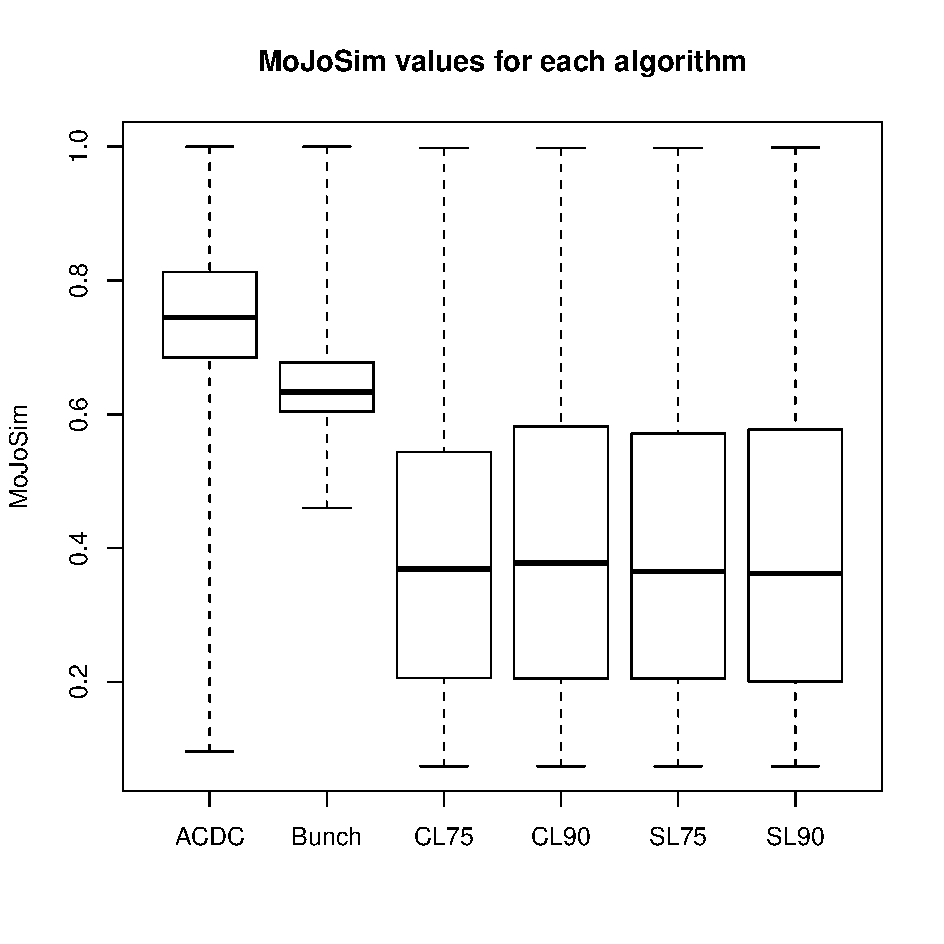
\includegraphics[width=0.5\textwidth]{figures/exp-algorithms}
		\caption{Statistical summary of MoJoSim values for each architecture recovery algorithm.}
		\label{fig:exp-algorithms}
	\end{figure}
	
	Another noteworthy aspect of the data is the dispersion of values. The algorithm Bunch presents the smaller dispersion, with more than half of the values between 0.60 and 0.80 (minimum value = 0.45). In the case of ACDC, half of the values are between 0.65 a 0.85, but the minimum value is 0.01. This observation suggests that, although Bunch presents overall inferior performance when compared with ACDC, it can be a reasonable choice for yielding more predictable results.
	
	\TODO move to a discussion section.
	The results disagree with conclusions from Wu, Hassah, and Holt \cite{Wu2005}. They have concluded that the SL algorithms outperform ACDC, which outperforms Bunch, which outperforms the CL algorithms. The disagreement probably can be explained by the criteria they used to build the reference architecture for each software system. They use the folder structure from the source of the software system to determine the modules in the architecture reference. In our work, the reference architecture is defined a priori, and the graphs are synthesized to reduce the dependencies between modules.
	
	We should note that this experiment suffers from sampling bias. Although all analyzeds graphs are software-realistic, we can not guarantee that it is representative of all software systems. We see this analysis as complementary to similar experiments, that suffer from other types of bias \cite{Wu2005,Bittencourt2009,Andritsos2005}.
	
\end{subsection}	

\begin{subsection}{Influence of the Number of Modules}
	% Section 6.5 from dissertation
	
	In the next experiment, we tried to understand how the algorithms behave on graphs with different number of modules. We were able to control the number of modules by changing the $G$ parameter for the BCR+ model.
	
	In this experiment, all graphs---both software-realistic and non software-realistic---were considered, in order to avoid the software-realism variable to bias the results.
	
	% We have analyzed the influence of the number of modules and of the proportion of external edges on the performance of the algorithms. We have chosen these two properties because they map naturally to BCR+ parameters: number of modules is controlled by the input module graph, $G$, and proportion of external edges is controlled by the parameter $\mu$.

	\TODO Move to experimental setup section?
	Because we have full control over the parameter values, the graphs can be paired, so the effect of each parameter can be isolated. For example, let $G$ be a graph in our data set that was synthesized using $\mu = 0.4$ and arbitrary values for the other parameters. There is another graph in the data set, $G\prime$, that was synthesized using the same parameter values as $G$, except for $\mu = 0.6$. Any observed difference between $G$ and $G\prime$ can be solely attributed to $\mu$ and to random effects. It should be noted that such pairing would not be possible in traditional approaches.
		
	% As expected, all algorithms performed better when the proportion of external edges was smaller. % I already checked the experimental package and found it to be true
	
	A surprising result was found when analyzing the influence of the number of modules on the performance of the algorithms (see Figure \ref{fig:exp-number-modules}). While the performance of ACDC and Bunch are not significantly influenced by the number of modules, the performance of the hierarchical algorithms is actually worse when applied to graphs with more modules. In fact, the performance of such algorithms are comparable to the performance of ACDC and Bunch when there are only two modules, but it gets  progressively worse as the number of modules grows.
	
	\begin{figure}[htbp]
		\centering
			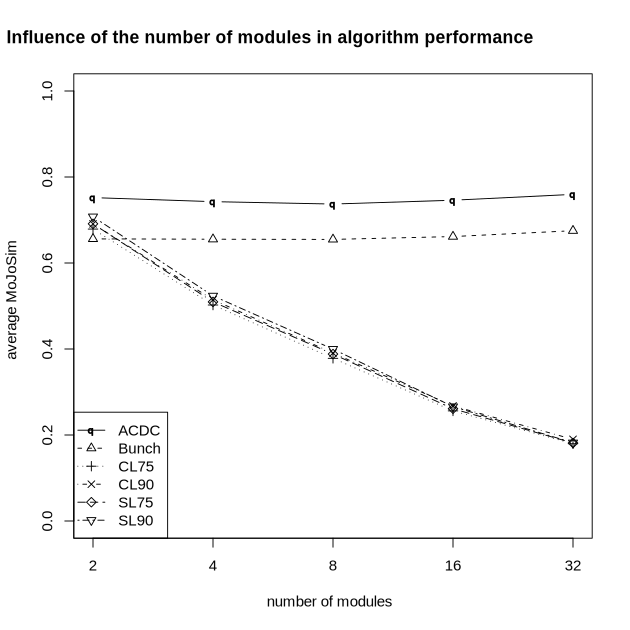
\includegraphics[scale=0.5]{figures/exp-number-modules}
		\caption{Influence of the number of modules in the reference architecture on the performance of each architecture recovery algorithm.}
		\label{fig:exp-number-modules}
	\end{figure}
	
	A possible explanation for this phenomenon can be found in the distribution of module sizes found by hierarchical algorithms. It is common that they found large modules, sometimes covering more than half of the vertices \cite{Wu2005}. If the reference architecture contains many smaller modules, large modules found by an algorithm are severely penalized by the MoJoSim metric (the large modules need to be split in smaller modules, which is accounted in MoJoSim as a sequence of vertex movements).
	
\end{subsection}

\begin{subsection}{Impact of Bidirectional Dependencies}
	% Section 6.6 from dissertation
	
	The third experiment was aimed at measuring the influence of the type of dependency (unidirectional of bidirectional) on the performance of each architecture recovery algorithm. The independent variable is the parameter $G$ from BCR+, that is, the definition of the modules and allowed dependencies between modules.
	
	We have analyzed two configurations for $G$:
	
	\begin{itemize}
		\item \emph{bidirectional}: $G$ contains two modules, $M_1$ and $M_2$; there is a bidirectional edge between $M_1$ and $M_2$ (that is, vertices in $M_1$ may depend on vertices of $M_2$ and the other way around);
		
		\item \emph{unidirectional}: $G$ contains two modules, $M_1$ and $M_2$; there is an unidirectional edge from $M_1$ to $M_2$ (that is, vertices in $M_1$ may depend on vertices of $M_2$, but the opposite is not true).
	\end{itemize}
	
	As far as we know, BCR+ is the only graph model that can be used to conduct this type of experiment. Other graph models do not offer control over specific dependencies.
	
	For the remaining parameters of BCR+, when considered the values described in Section XXX. For each configuration of parameters, three graphs were synthesized, totalizing 11,400 graphs. Then, each architecture recovery algorithm was applied to each graph. Finally, the performance was computed, using the metric MoJoSim.
	
	The results are shown in a box plot in Figure \ref{fig:exp-dependencies}. It can be observed that all algorithms performed slightly better on the graph with the unidirectional edge. All differences---except that of CL75---are significative at 5\% level, as assessed with the paired Wilcoxon test.
	
	\begin{figure*}[htbp]
		\centering
			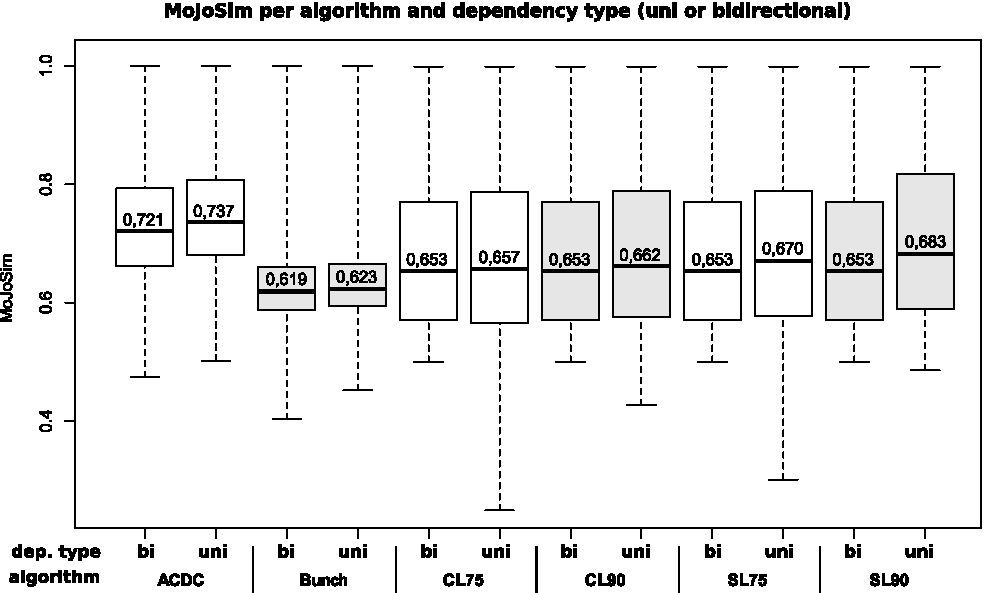
\includegraphics[scale=1]{figures/exp-dependencies}
		\caption{Influence of the type of dependency between modules (unidirectional or bidirectional) on the performance of each architecture recovery algorithm.}
		\label{fig:exp-dependencies}
	\end{figure*}
	
	The difference of performance for each algorithm is shown in Table \ref{tab:exp-dependencies}, as a 95\% confidence interval. ACDC and SL75 are more influenced by the choice of dependency type than the other algorithms. Overall, the difference between MoJoSim values does not exceed 0.03 (except in the case of SL90), which is a small value.
	
	\begin{table*}[width=\textwidth]
	  \begin{center}
	  \begin{tabular}{cccccc}
	    \hline
	    \textbf{ACDC} & \textbf{Bunch} & \textbf{CL75} & \textbf{CL90} & \textbf{SL75} & \textbf{SL90} \\
	    \hline
	    \hline
	    \footnotesize{[0,016; 0,023]} & \footnotesize{[0,004; 0,008]} & \footnotesize{[-0,004; 0,006]} & \footnotesize{[0,006; 0,015]} & \footnotesize{[0,007; 0,017]} & \footnotesize{[0,021; 0,031]} \\
	    \hline
	  \end{tabular}
	  \end{center}
	  \caption{95\% confidence interval for the performance difference for each algorithm, measured by MoJoSim, between uni- and bidirectional intermodule dependencies.}
	  \label{tab:exp-dependencies}
	\end{table*}

	% We conclude that, in general, the presence of modules with mutual, bidirectional dependencies, influences negatively the performance of the algorithms that were analyzed. 
	
	The difference in performance is negligible, unlikely to be relevant in practical terms. Therefore, we conclude that the algorithms are robust with respect of mutual intermodule dependencies.
	
	% We conclude that, in general, the presence of modules with mutual, bidirectional dependencies, influences negatively the performance of the algorithms that were analyzed. The observed difference was small in our study with two modules, but we suspect that this difference can be greater on graphs with more modules and more bidirectional dependencies.
	
\end{subsection}

\begin{subsection}{Discussion}
  % TODO: move to a new section
	We have described three experiments based on the application of architecture recovery algorithms to synthetic graphs created by the model BCR+. The experiments present evidence that this approach is practicable and can be used to find insights about the algorithms that cannot be found with more traditional approaches.
	
	\TODO more
	
\end{subsection}

\end{section}

%%%%%%%%%%%%%%%%%%%%%%%%%%%%%%%%%%%%%%%%%%%%%%%%%%%%%%%%%%%%%%%%%%%%%%%%%%%%%

\begin{section}{Other Possible Sections}
	Discussion
	
	Limitations: selection bias for training the classifier. selection bias for synthesized graphs.
	
	Related work: evaluation of Bunch using random graphs. Lancichinetti's evaluation of clustering algorithms using his network model. Evaluation of architecture recovery algorithms by comparing recovered modules with packages that are explicit in source code. (TODO: maybe promote to 2nd section)
	
	Conclusion
	
	Acknowledgments
	
	References	
	
	\TODO Publish the benchmark as a SQLite database, along with documentation and scripts.
	
\end{section}

%%%%%%%%%%%%%%%%%%%%%%%%%%%%%%%%%%%%%%%%%%%%%%%%%%%%%%%%%%%%%%%%%%%%%%%%%%%%%
%%%%%%%%%%%%%%%%%%%%%%%%%%%%%%%%%%%%%%%%%%%%%%%%%%%%%%%%%%%%%%%%%%%%%%%%%%%%%

\bibliographystyle{plain}
\bibliography{ase2012-reference-arch}

\end{document}
